\documentclass[a4paper, 11pt]{article}
\usepackage{geometry}
 \geometry{
 a4paper,
 total={170mm, 257mm},
 left=20mm,
 top=20mm,
 }
\usepackage[english]{babel}
\usepackage[T1]{fontenc}
\usepackage[latin1]{inputenc}
\usepackage{fancyhdr}
\usepackage{float}
\usepackage{placeins}
\usepackage{graphicx}
\usepackage{caption}
\usepackage{subcaption}
\graphicspath{{../plots/}}
%\graphicspath{{../plots_gpu/}}
\DeclareGraphicsExtensions{.pdf,.png,.jpg}
\usepackage{pdflscape}
\usepackage{wrapfig}
\usepackage{amsfonts}

\usepackage{amsmath}
\usepackage{amssymb}
%\DeclareMathOperator*{\argmax}{argmax}
%\DeclareMathOperator*{\argmin}{argmin}
\DeclareMathOperator*{\argmax}{arg\,max}
\DeclareMathOperator*{\argmin}{arg\,min}

\usepackage{algpseudocode}
\usepackage{mathtools}

\DeclarePairedDelimiter{\ceil}{\lceil}{\rceil}
\DeclarePairedDelimiter{\floor}{\lfloor}{\rfloor}

\begin{document}

\section{Theoretical model}
A hypotethical serial algorithm reads $N \in \mathbb{N}$ numbers in $T_{read}$ seconds and computes their sum in $T_{comp} \times (N-1)$ seconds. Thus the total time spent is
$$T_{serial}(N) = T_{read} + (N-1)T_{comp}$$
A naive MPI algorithm for the same task, given $P \geq 1, P \in \mathbb{N}$ processes divided in one master and $P-1$ slaves, reads the numbers on the master and distributes serially $P-1$blocks of at most $\ceil{N/P}$ elements to the slaves. Each process performs the $\ceil{N/P}-1$ sums on its respective block, the partial results are then collected and summed serially by the master.\\
%\begin{itemize}
%\item the master reads the $N$ numbers in $T_{read}$ seconds
%\item the master splits the numbers in $P$ blocks of at most $\ceil{N/P}$ elements and distributes $P-1$ blocks one to each slave, in $(P-1)T_{comm}$ seconds
%\item each process computes the sum of its block of numbers in $\left(\ceil{N/P}-1\right)T_{comp}$ seconds
%\item each slave sends its result to the master, which receives them serially in $(P-1)T_{comm}$ seconds
%\item the master computes the final sum in $(P-1)T_{comp}$ seconds
%\end{itemize}
The time to retrieve the result is then:
$$T_{naive}(N, P) \leq T_{read} + 2(P-1)T_{comm} + \left(\ceil[\bigg]{\frac{N}{P}}+P-2\right)T_{comp}$$
If $P=1$, there is no difference with the serial approach.\\
The following numerical evaluation assume $T_{read} = 10^{-4}$ s, $T_{comp} = 2 \times 10^{-9}$ s and $T_{comm} = 10^{-6}$ s.
%\begin{itemize}
%\item $T_{read} = 10^{-4}$ s
%\item $T_{comp} = 2 \times 10^{-9}$ s
%\item $T_{comm} = 10^{-6}$ s
%\end{itemize}
Under these assumptions, communication time is independent of message size.\\
\subsection{Scalability of the naive algorithm}
Defining scalability as
$$S_{naive}(N, P) = \frac{T_{naive}(N, 1)}{T_{naive}(N, P)}$$
%\begin{figure}[h]
%    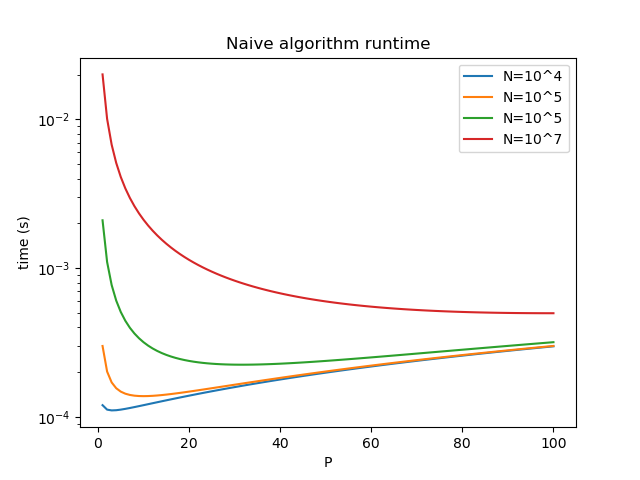
\includegraphics[width=11cm]{theoretical_naive_time}
%    \caption{Time of the naive algorithm}
%\end{figure}
%\begin{figure}[h]
%    \includegraphics[width=11cm]{theoretical_naive_scalability}
%    \caption{Scalability of the naive algorithm}
%\end{figure}
\FloatBarrier
\begin{figure}[h]
\centering
\begin{minipage}{.5\textwidth}
  \centering
  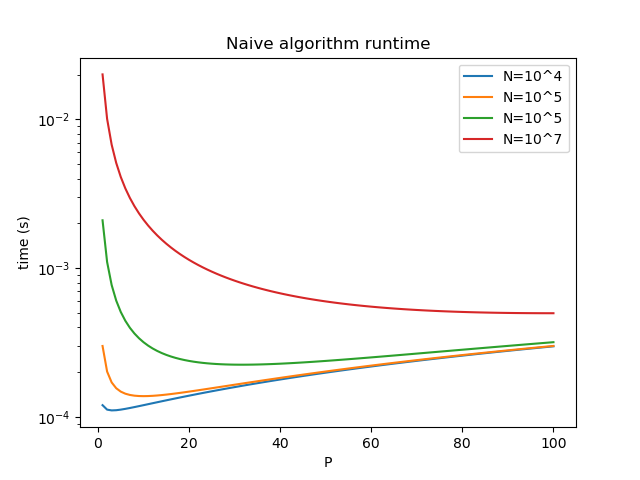
\includegraphics[width=\linewidth]{theoretical_naive_time}
  \captionof{figure}{Time of the naive algorithm}
  \label{fig:theoretical_naive_time}
\end{minipage}%
\begin{minipage}{.5\textwidth}
  \centering
  \includegraphics[width=\linewidth]{theoretical_naive_scalability}
  \captionof{figure}{Scalability of the naive algorithm}
  \label{fig:theoretical_naive_scalability}
\end{minipage}
\end{figure}
\FloatBarrier
The graphs show that scalability is not perfect; the naive algorithm scales only when $P$ is small compared to $N$, then scalability peaks and decreases.\\
Maximum scalability is achieved by $N, P_{opt}$ such that $T_{naive}(N, P_{opt})$ is at its mininum given $N$.\\
Ignoring the ceiling on the block size, taking the derivative with respect to $P$ and finding its root $P_{*}$:
%$$\frac{\partial T_{naive}(N, P)}{\partial P} = 2T_{comm} + \left(1-\frac{N}{P^{2}}\right)T_{comp}$$
%$$2T_{comm} + \left(1-\frac{N}{P_{*}^{2}}\right)T_{comp} = 0$$
$$P_{*} = \sqrt{N\frac{T_{comp}}{2T_{comm} + T_{comp}}}$$
The second derivative is strictly positive, so $P_{*}$ determines a minimum for $T_{naive}$ and a maximum for $S_{naive}$.\\
%$$\frac{\partial^{2} T_{naive}(N, P)}{\partial P^{2}} = \frac{N2T_{comp}}{P^{3}} > 0$$
Recalling the domain of $P$, one still needs to consider floor and ceiling of $P_{*}$
$$P_{opt}(N) = \argmin_{P \in \{ \floor{P_{*}}, \ceil{P_{*}} \}, P \geq 1 }{T_{naive}(N, P)} $$\\
The derivative with respect to $N$ is strictly positive and there is no stationary point.\\
%The derivative with respect to $N$ is $T_{comp}/P > 0$, there is no stationary point.\\
\subsection{Enhanced algorithm}
A different algorithm can exploit the system's parallelism by distributing the burden of communications across the processes, so that they can be performed in parallel rather than serially.\\
Let the master process have rank $0$ and the slaves have ranks $1$ through $P-1$.\\
Rank $0$ sends a message to rank $\ceil*{P/2}$, containing $\floor*{P/2}$ blocks of at most $\ceil{N/P}$ numbers. The problem then reduces to two instances of size $P_{0}=\ceil*{P/2}$ and $P_{1}=\floor*{P/2}$, of which ranks $0$ and $\ceil*{P/2}$ are the respective masters.\\
The two instances can proceed in parallel until every process either has received a single block, or has sent all but one, at which point computation of the block's sum can be performed in parallel.\\
The first communication phase requires $\ceil*{\log_{2}(P)}$ steps and completes in $\ceil*{\log_{2}(P)}T_{comm}$ seconds.\\
Collection of the results will use the opposite schema, but the message will contain the partial result and the reveicer will sum it with its own; it will complete in $\ceil*{\log_{2}(P)}(T_{comm} + T_{comp})$ seconds.\\
As data are read like in the naive algorithm and each process computes the sum for a block of the same size, the algorithm completes in
$$T_{enh}(N, P) \leq T_{read} + \ceil*{\log_{2}(P)} (2T_{comm} + T_{comp}) + \left(\ceil[\bigg]{\frac{N}{P}}-1\right)T_{comp}$$
%\begin{figure}[h]
%    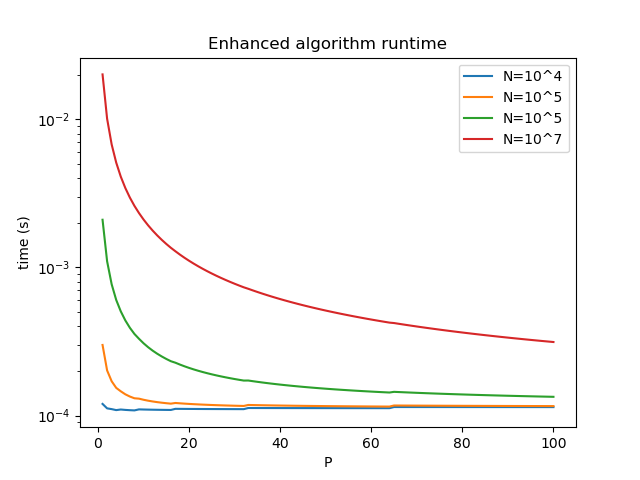
\includegraphics[width=12cm]{theoretical_enhanced_time}
%    \caption{Time of the enhanced algorithm}
%\end{figure}
%\begin{figure}[h]
%    \includegraphics[width=12cm]{theoretical_enhanced_scalability}
%    \caption{Scalability of the enhanced algorithm}
%\end{figure}
\begin{figure}[h]
\centering
\begin{minipage}{.5\textwidth}
  \centering
  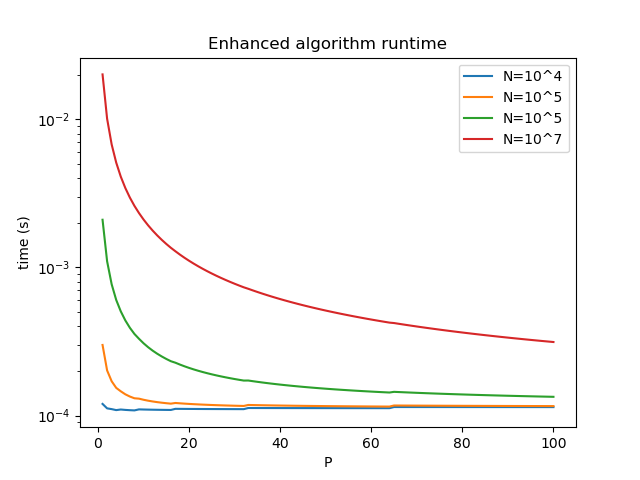
\includegraphics[width=\linewidth]{theoretical_enhanced_time}
  \captionof{figure}{Time of the enhanced algorithm}
  \label{fig:theoretical_enhanced_time}
\end{minipage}%
\begin{minipage}{.5\textwidth}
  \centering
  \includegraphics[width=\linewidth]{theoretical_enhanced_scalability}
  \captionof{figure}{Scalability of the enhanced algorithm}
  \label{fig:theoretical_enhanced_scalability}
\end{minipage}
\end{figure}
%\FloatBarrier
The graphs show the effect of the ceiling function on the logarithm, with a sharp increase in time when $P$ passes from a power of 2 to the next value. This effect is negligible when $(N/P)T_{comp} \gg \log_{2}(P)T_{comm}$ \\
Proceeding as for the naive algorithm, by relaxing integrality and taking the derivative with respect to $P$:
%Having reduced the communication time to an asymptotically sub-linear function of $P$ greatly benefits the scalability, for which the $P_{opt}(N)$ is linear in $N$.\\
%Indeed, relaxing the ceiling function:
%$$\frac{\partial T_{enh}(N, P)}{\partial P} = \frac{2T_{comm} + T_{comp}}{\ln(2)P} -\frac{N}{P^{2}} T_{comp}$$
%$$\frac{2T_{comm} + T_{comp}}{\ln(2)P_{*}} - \frac{N}{P_{*}^{2}} T_{comp} = 0$$
$$P_{*} = N\ln(2)\frac{T_{comp}}{2T_{comm} + T_{comp}}$$
Restoring integrality yields
$$P_{opt}(N) = \argmin_{P \in \{ 2^{\floor{\log_2(P_{*})}}, 2^{\ceil{\log_2(P_{*})}} \}, P \geq 1}{T_{enh}(N, P)} $$\\
Peak scalability is reached for much greater values of $P$ than with the naive algorithm.\\
\section{MPI program}
Two programs for the estimation of $\pi$ using a Monte-Carlo method have been provided, \texttt{pi.c} and \texttt{mpi\_pi.c}; the first being a serial implementation, the second using MPI.\\
Both programs take as input $N$, the number of iterations.\\
The serial program uses \texttt{clock()} from \texttt{time.h} to measure the processor time elapsed from initialization of the random generator to output of the estimate.\\
The MPI program adopts a master-slave approach where each process computes $\floor{N/P}$ iterations, then each slave sends its result to the master and exits; the master finally computes the estimate. Communications between processes are blocking and the master receives partial sums in sequential order of slaves' ranks.\\
The MPI program uses \texttt{MPI\_Wtime} to measure the elapsed wall time. The master counts from initialization of the random generator to output of the final estimate, thus including the (blocking) receival of each slave's partial sum.\\
Slaves count from initialization of the random generator to the conclusion of the communication with the master.\\
The MPI program is executed through \texttt{mpirun} and it is not possible to make assumptions on the actual starting order of the processes. The extremes of the measured intervals can be interleaved in any possible combination.\\
%Lastly, the two programs use different seeds for the random generator and this can impact the behavior of the main loop, whose body comprises a conditional.
All the following timings have been obtained on Orfeo's gpu nodes, each equipped with a pair of Intel Xeon Gold 6226 providing a total of 48 virtual threads due to Hyper-Threading.
\subsection{Strong scalability}
Using \texttt{/usr/bin/time}'s elapsed measurement, the serial program performs $N=10^8$ iterations in 2.583s on average, with no system time. Under the same workload, the MPI program with a single process takes on average 2.873s, of which 0.123s are spent as system time.\\
The overhead is mainly due to the \texttt{mpirun} call, which is responsible for the system time spent in spawning the children process and output collection and a minor component in user space. Indeed, the internal times reported by the two programs are close: 2.567s for the serial version, 2.589s for the MPI version.\\
%When increasing the number of iterations, the variability of system time for the MPI program grows while the minimum remains about constant. This suggests that \texttt{mpirun} randomly conflicts with its child process.\\ 
%\begin{tabular}{ l c r }
%  1 & 2 & 3 \\
%  4 & 5 & 6 \\
%  7 & 8 & 9 \\
%\end{tabular}
The internal times provided by the two programs differ in that the MPI program includes the communication between master and slaves. The maximum time across all processes constitutes the worst case; it is usually found on the master process, but due to the unpredictability of process starting order and communication time, it is possible for slaves to measure higher times.\\
%The internal time can be used to study the scalability of the single code segment, while the elapsed time pertains the 
%Considering the elapsed time as the performance metric with which scalability is studied, 
The components identified above are independent of $N$ and their influence is mitigated when increasing the workload.\\
%Comparison of the worst case internal times excludes the overhead from \texttt{mpirun}.
The following plots compare the two timing methods in a strong scaling experiment, with $P \in \{ 1,4,8,\ldots,48 \}$ and $N=10^{8}$.\\
\begin{figure}[h]
\centering
\begin{minipage}{.5\textwidth}
  \centering
  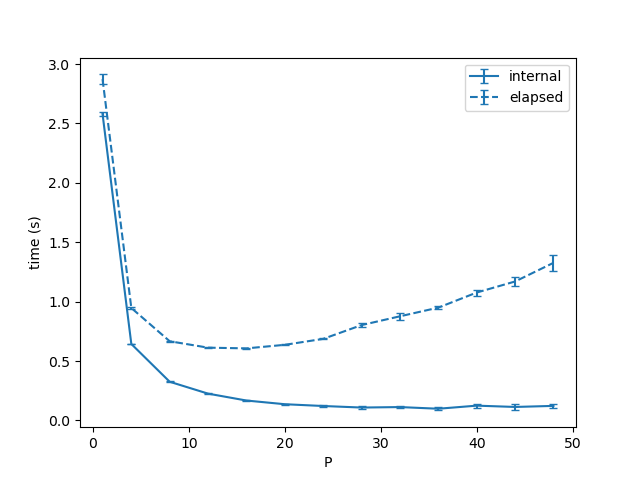
\includegraphics[width=\linewidth]{strong_scalability_time_compare}
  \captionof{figure}{Strong scalability times ($N=10^{8}$)}
  \label{fig:strong_scalability_time_compare}
\end{minipage}%
\begin{minipage}{.5\textwidth}
  \centering
  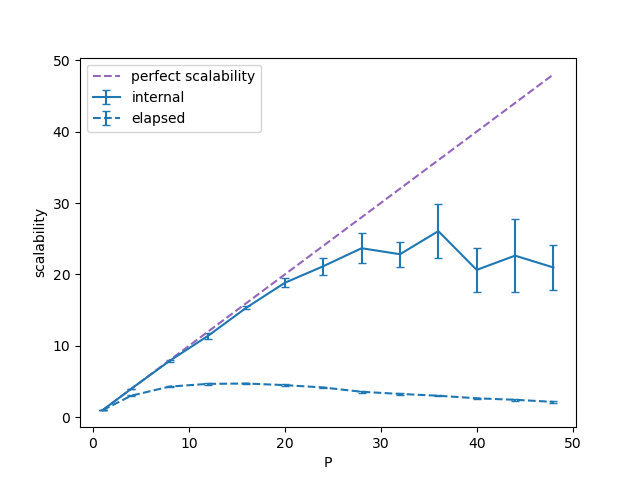
\includegraphics[width=\linewidth]{strong_scalability_scalability_compare}
  \captionof{figure}{Strong scalability ($N=10^{8}$)}
  \label{fig:strong_scalability_scalability_compare}
\end{minipage}
\end{figure}
Internal time resembles the expected hyperbole, but elapsed time seems to asymptotically grow linearly with $P$.\\
The difference between elapsed and internal time is due to \texttt{mpirun} and the variability in starting and ending times of the single processes. This overhead grows with the number of processors due to the spawning of $P$ processes and quickly dominates the curve's behavior as the main loop's workload decreases.\\
%determines the tail behavior due to cost of such operation dominating the  $\floor{N/P}$ steps of the process' main loops.\\
Elapsed time reaches its minimum for $P=12$; the penalty in scalability is severe due to the overhead quickly outgrowing the actual computation time of the loop.\\
Internal time still includes a communication section whose steps linearly increase with $P$, although its effect is much smaller than the overhead. Minimum time is found for $P=36$ and scalability declines, although in that interval experimental variability is conspicuous.\\
Overall, the plots reflect the theoretical model seen for the naive MPI algorithm in the initial section.\\
The experiment has been integrated with measures for $N=10^{9}, 10^{10}, 10^{11}$.
\begin{figure}[h]
\centering
\begin{minipage}{.5\textwidth}
  \centering
  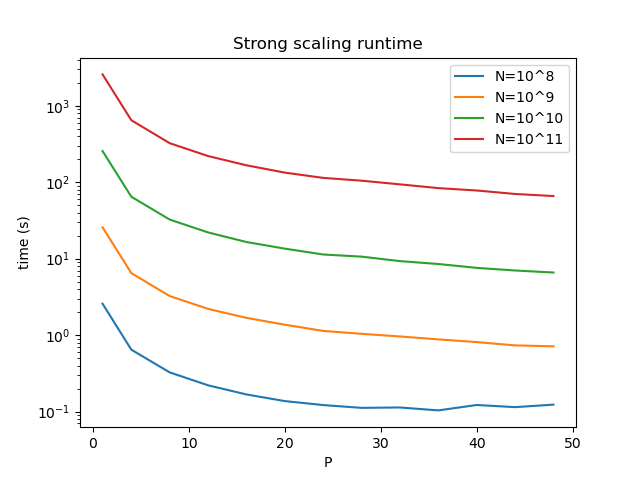
\includegraphics[width=\linewidth]{strong_scalability_internal}
  \captionof{figure}{Strong scaling (internal time)}
  \label{fig:strong_scalability_internal}
\end{minipage}%
\begin{minipage}{.5\textwidth}
  \centering
  \includegraphics[width=\linewidth]{strong_scalability_internal_scalability}
  \captionof{figure}{Strong scalability (internal time)}
  \label{fig:strong_scalability_internal_scalability}
\end{minipage}
\end{figure}
%choose timing method
\begin{figure}[h]
\centering
\begin{minipage}{.5\textwidth}
  \centering
  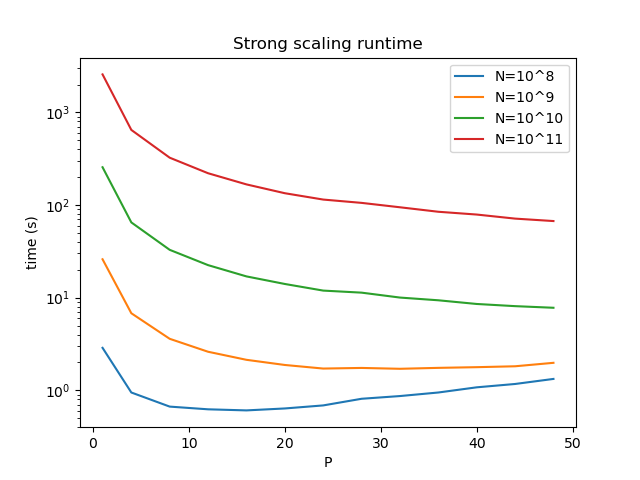
\includegraphics[width=\linewidth]{strong_scalability_elapsed}
  \captionof{figure}{Strong scaling (elapsed time)}
  \label{fig:strong_scalability_elapsed}
\end{minipage}%
\begin{minipage}{.5\textwidth}
  \centering
  \includegraphics[width=\linewidth]{strong_scalability_elapsed_scalability}
  \captionof{figure}{Strong scalability (elapsed time)}
  \label{fig:strong_scalability_elapsed_scalability}
\end{minipage}
\end{figure}
%Increasing $N$ reduces the effect of \texttt{mpirun}'s overhead.\\
Scalability of heaviest workloads highlight a discontinuity between the behavior for $P \leq 24$ and $P > 24$, with a steeper decrease in the latter. This can be explained by the activation of Hyper-Threading, since at $P > 24$ at least two processes must share the same physical core, thus sharing the execution resources and increasing the execution time.\\
A single shared core is sufficient to manifest this slowdown, due to the blocking MPI directives being used.\\
Except for $N=\0^{8}$, 
\subsection{Parallel overhead model}

\subsection{Weak scalability}
The experiment on weak scalability has been performed with $N=10^{8}, 10^{9}, 10^{10}$ and $P=1, 4, \ldots , 48$, and $N=10^{11}$ with $P=1, 12, 24, 48$.\\
The runtime increases with the number of processors, which is consistent with the previous observations of overhead modeling. The slope of the function changes for $P > 24$, due to the interference between processes in Hyper-Threading cores; this effect is masked by the reduced number of cores used for $N=10^{11}$.
\begin{figure}[h]
\centering
\begin{minipage}{.5\textwidth}
  \centering
  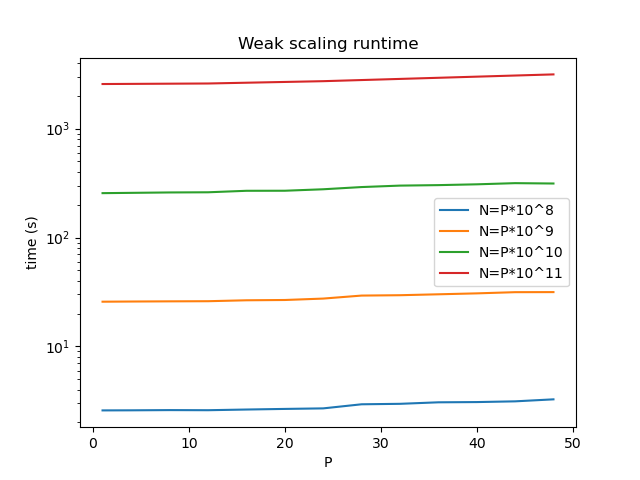
\includegraphics[width=\linewidth]{weak_scalability_internal}
  \captionof{figure}{Weak scaling (internal time)}
  \label{fig:weak_scalability_internal}
\end{minipage}%
\begin{minipage}{.5\textwidth}
  \centering
  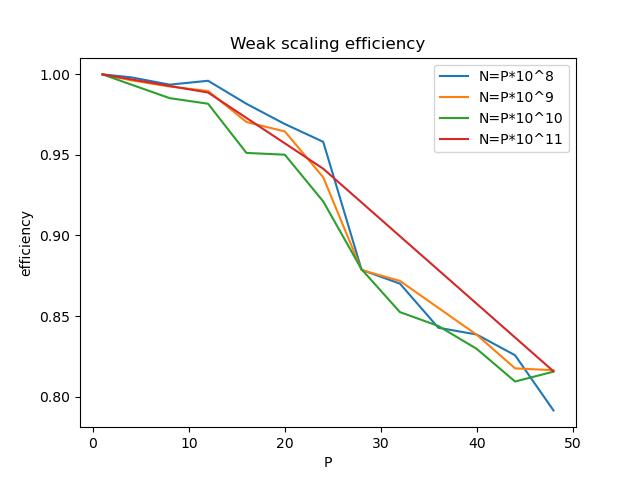
\includegraphics[width=\linewidth]{weak_scalability_internal_efficiency}
  \captionof{figure}{Weak efficiency (internal time)}
  \label{fig:weak_scalability_internal_efficiency}
\end{minipage}
\end{figure}
%choose timing method
\begin{figure}[h]
\centering
\begin{minipage}{.5\textwidth}
  \centering
  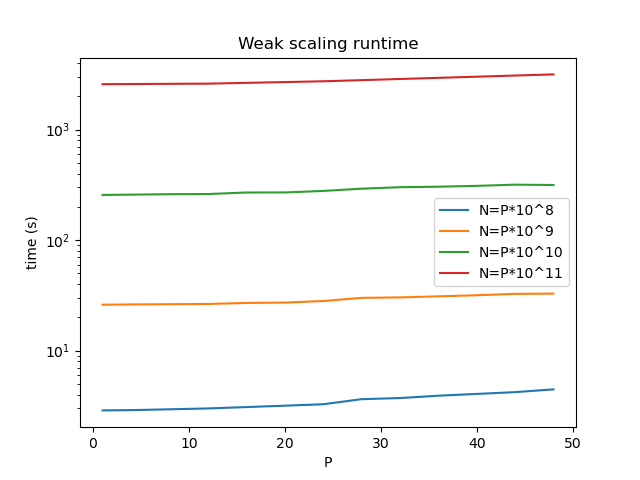
\includegraphics[width=\linewidth]{weak_scalability_elapsed}
  \captionof{figure}{Weak scaling (elapsed time)}
  \label{fig:weak_scalability_elapsed}
\end{minipage}%
\begin{minipage}{.5\textwidth}
  \centering
  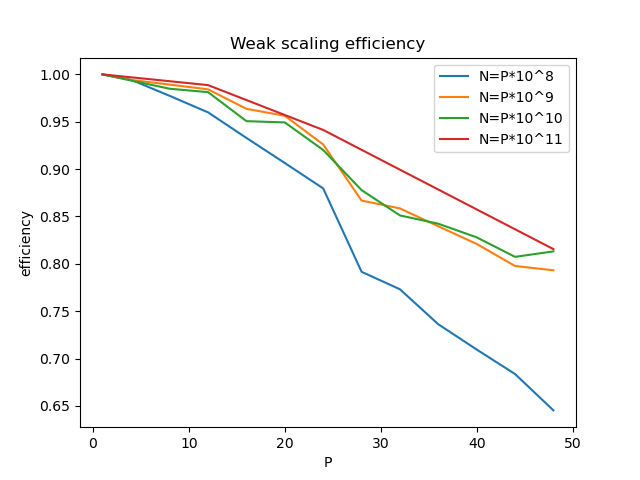
\includegraphics[width=\linewidth]{weak_scalability_elapsed_efficiency}
  \captionof{figure}{Weak efficiency (elapsed time)}
  \label{fig:weak_scalability_elapsed_efficiency}
\end{minipage}
\end{figure}
\end{document}